\documentclass{article}
\usepackage{beamerarticle}
\setjobnamebeamerversion{toolkit-b}

\usepackage{fullpage}

\usepackage[backend=biber,url=false,style=alphabetic]{biblatex}
\addbibresource{os.bib}

\usepackage{hyperref}
\usepackage[textsize=footnotesize]{todonotes}
\addtolength{\oddsidemargin}{-15pt}
\addtolength{\marginparsep}{5pt}
% \setlength{\marginparwidth}{1.2in}
% \let\oldmarginpar\marginpar
% \renewcommand\marginpar[1]{\-\oldmarginpar[\raggedleft\footnotesize #1]%
% {\raggedright\footnotesize #1}}
\newcommand{\Marginpar}[1]{\marginpar{\raggedright{\footnotesize \emph{#1}}}}

% http://tex.stackexchange.com/q/25259/86
% for *notes*
\defbeamertemplate<article>{frame begin}{lined}{
  \par\noindent\rule{\textwidth}{2pt}\par}
\defbeamertemplate<article>{frame end}{lined}{
  \par\vspace{1em}\noindent\rule{.1\textwidth}{.3pt}
  \raisebox{-3pt}{{\large \Info}}
  \rule{.1618\textwidth}{.3pt}\par\vspace{.5em}}

\setbeamertemplate{frame begin}[lined]
\setbeamertemplate{frame end}[lined]

\mode*

\lecture[toolkit]{toolkit}{toolkit}

\section{Before Diving Into The Kernel Source}

\subsection{Getting Started with the Kernel}

Ref: \citetitle[Chapter 2, \emph{Getting Started with the Kernel}]{love2010linux}

\begin{frame}[fragile=singleslide]{Obtaining The Kernel Source}
  \begin{itemize}
  \item[Web:] \url{http://www.kernel.org}
  \item[Git:] Version control system
  \end{itemize}
  {\scriptsize
    \begin{itemize}
    \item[\$] \texttt{git clone git://git.kernel.org/pub/scm/linux/kernel/git/torvalds/linux-2.6.git}
    \end{itemize}}
\end{frame}

\begin{frame}{Installing The Kernel Source}
  In \texttt{/usr/src/} directory:
  \begin{itemize}
  \item[\$] \texttt{tar xvjf linux-x.y.z.tar.bz2}
  \item[\$] \texttt{tar xvzf linux-x.y.z.tar.gz}
  \item[\$] \texttt{xz -dc linux-x.y.z.tar.xz | tar xf -}
  \item[\$] \texttt{ln -s linux-x.y.z linux}
  \end{itemize}
  ``\texttt{sudo}'' if needed.
\end{frame}

\begin{frame}{The Kernel Source Tree}
  \begin{center}
    \begin{scriptsize}{\ttfamily
      \begin{tabular}{ll}
        arch& Architecture-specific source\\
        block& Block I/O layer\\
        crypto& Crypto API\\
        Documentation& Kernel source documentation\\
        drivers& Device drivers\\
        firmware& Device firmware needed to use certain drivers\\
        fs& The VFS and the individual filesystems\\
        include& Kernel headers\\
        init& Kernel boot and initialization\\
        ipc& Interprocess communication code\\
        kernel& Core subsystems, such as the scheduler\\
        lib& Helper routines\\
        mm& Memory management subsystem and the VM\\
        net& Networking subsystem\\
        samples& Sample, demonstrative code\\
        scripts& Scripts used to build the kernel\\
        security& Linux Security Module\\
        sound& Sound subsystem\\
        usr& Early user-space code (called initramfs)\\
        tools& Tools helpful for developing Linux\\
        virt& Virtualization infrastructure\\
      \end{tabular}}
    \end{scriptsize}
  \end{center}
  \begin{itemize}
    \item[\$] \texttt{tree /usr/src/linux}
  \end{itemize}
\end{frame}

\begin{frame}{Building The Kernel}
  \begin{block}{Configuration}
    \begin{center}
      \texttt{make config | make menuconfig | make gconfig}
    \end{center}
    \begin{itemize}
    \item[\$] \texttt{make defconfig \emph{\# Defaults}}
    \item[\$] \texttt{make oldconfig \emph{\# Using .config file}}
    \end{itemize}
  \end{block}
  \begin{block}{Make}
    \begin{itemize}
    \item[\$] \texttt{make -jN > /dev/null}
      \begin{itemize}
      \item[N:] number of jobs. Usually one or two jobs per processor.
      \end{itemize}
    \end{itemize}
  \end{block}
\end{frame}

\begin{frame}
  \begin{block}{Installing The New Kernel}
    \begin{itemize}
    \item[\$] \texttt{sudo make modules\_install}
    \item[\$] \texttt{sudo make install}
    \end{itemize}
    \texttt{grub2} config should be updated automatically. Check
    \begin{itemize}
    \item \texttt{/etc/grub.d/}
    \item \texttt{/boot/grub/grub.cfg}
    \end{itemize}
    ``\texttt{sudo reboot}'' to try your luck.
  \end{block}
\end{frame}

See also: \citetitle{web:debkernelhandbook}

\subsection{A Beast Of A Different Nature}

\begin{frame}\mode<beamer>{\frametitle{A Beast Of A Different Nature}}
  \begin{itemize}
  \item Neither the C library nor the standard C headers
  \item GNU C
  \item Lack of memory protection
  \item No floating-point operations
  \item Small per-process fixed-size stack
  \item Synchronization and concurrency
  \item Portability
  \end{itemize}
\end{frame}

\begin{frame}
  \begin{block}{No libc or standard headers}
    \begin{itemize}
    \item Chicken-and-the-egg situation
    \item Speed and size
    \end{itemize}
    Many of the usual libc functions are implemented inside the kernel. For example,
    \begin{itemize}
    \item String operation: \texttt{lib/string.c}, \texttt{linux/string.h}
    \item \texttt{printk()}
    \end{itemize}
  \end{block}
\end{frame}

\begin{frame}{GNU C}
  The kernel developers use both \texttt{ISO C99} and \texttt{GNU C} extensions to the C
  language.
  \begin{itemize}
  \item Inline functions
  \item Inline assembly
  \end{itemize}
\end{frame}

\begin{frame}[fragile=singleslide]
  \begin{block}{Inline functions}
    Inserted inline into each function call site
    \begin{itemize}
    \item[\good] eliminates the overhead of function invocation and return (register saving and
      restore)
    \item[\good] allows for potentially greater optimization
      % as the compiler can optimize both the caller and the called function as one
    \item[\bad] code size increases
    \end{itemize}
  \end{block}
  \begin{center}
  \begin{ccode}
static inline void wolf(unsigned long tail_size)
\end{ccode}
  \end{center}
  \begin{itemize}
  \item Kernel developers use inline functions for small time-critical functions
  \item The function declaration must precede any usage
    \begin{description}
    \item[Common practice:] place inline functions in header files
    \end{description}
  \end{itemize}
\end{frame}

See also:
\begin{itemize}
\item \citetitle{wiki:inlinefunction}
\item \citetitle{web:inline-c}
\end{itemize}

\begin{frame}[fragile=singleslide]
  \begin{block}{Inline assembly}
    Embedding assembly instructions in normal C functions
    \begin{itemize}
    \item[\good] speed
    \item[\bad] Architecture dependent (poor potability)
    \end{itemize}
  \end{block}
  \begin{block}{Example: Get the value from the timestamp(tsc) register}
    \begin{center}
\begin{ccode}
unsigned int low, high;
asm volatile("rdtsc" : "=a" (low), "=b" (high));
\end{ccode}
    \end{center}
  \end{block}
\end{frame}

See also: \citetitle{wiki:inline-asm}

\begin{frame}[fragile=singleslide]
  \begin{block}{Branch prediction}
    The \texttt{likely()} and \texttt{unlikely()} macros allow the developer to tell the CPU,
    through the compiler, that certain sections of code are likely, and thus should be
    predicted, or unlikely, so they shouldn't be predicted.
  \end{block}
  \begin{center}
\begin{ccode}
#define   likely(x)  __builtin_expect(!!(x),1)
#define unlikely(x)  __builtin_expect(!!(x),0)
\end{ccode}
  \end{center}
  \begin{block}{Example: \texttt{kernel/time.c}}
    \begin{center}
      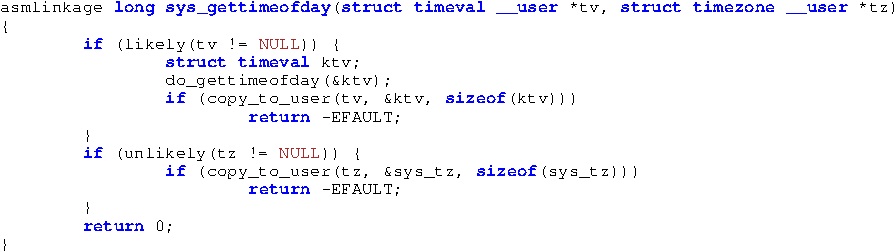
\includegraphics[width=\textwidth]{time}
    \end{center}
  \end{block}
\end{frame}

In this code, we see that a syscall to get the time of day is likely to have a
\texttt{timeval} structure that is not null. If it were null, we couldn't fill in the
requested time of day! It is also unlikely that the timezone is not null. To put it
another way, the caller rarely asks for the timezone and usually asks for the time.
\citetitle[Sec.~2.8.2, \emph{\texttt{likely()} and \texttt{unlikely()}}]{rodriguez2005linux}

\begin{description}
\item[\texttt{!!(x)}] make sure \texttt{x} is a boolean variable, since in C, macro
  invocations do not perform type checking, or even check that arguments are
  well-formed. 
\end{description}

See also:
\begin{itemize}
\item \citetitle{web:likely}
\item \citetitle{wiki:inlinefunction}
\end{itemize}

\begin{frame}
  \begin{block}{No memory protection}
    \begin{itemize}
    \item Memory violations in the kernel result in an \emph{oops}
    \item Kernel memory is not pageable
    \end{itemize}
  \end{block}
\end{frame}

See also: \citetitle{wiki:kernel-oops}.

\begin{frame}
  \begin{block}{No (easy) use of floating point}
    \begin{itemize}
    \item rarely needed
    \item expensive: saving the FPU registers and other FPU state takes time
    \item not every architecture has a FPU, e.g. those for embedded systems
    \end{itemize}
  \end{block}
\end{frame}

See also:
\begin{itemize}
\item \citetitle{web:kernel-fp}
\item \citetitle{web:kernel-fp2}
\end{itemize}

\begin{frame}
  \begin{block}{Small, fixed-size stack}
    \begin{itemize}
    \item On x86, the stack size is configurable at compile time, 4K or 8K (1 or 2 pages)
    \end{itemize}
  \end{block}
\end{frame}

\subsection{Common Kernel Data-types}

\begin{itemize}
\item \citetitle[Chapter 2, \emph{Exploration Toolkit}]{rodriguez2005linux};
\item \citetitle[Chapter 6, \emph{Kernel Data Structures}]{love2010linux}; 
\item \citetitle[Chapter 11, \emph{Data Types in the Kernel}]{corbet05ldd}
\end{itemize}

\begin{frame}{Data Types in the Kernel}
  Three main classes:
  \begin{enumerate}
  \item Standard C types, e.g. \texttt{int}
  \item Explicitly sized types, e.g. \texttt{u32}
  \item Types used for special kernel objects, e.g. \texttt{pid\_t}
  \end{enumerate}
\end{frame}

Although you must be careful when mixing different data types, sometimes there are good
reasons to do so. One such situation is for memory addresses, which are special as far as
the kernel is concerned. Although, conceptually, addresses are pointers, \emph{memory
administration is often better accomplished by using an unsigned integer type; the
  kernel treats physical memory like a huge array, and a memory address is just an index
  into the array. Furthermore, a pointer is easily dereferenced; when dealing directly
with memory addresses, you almost never want to dereference them in this manner. Using an
integer type prevents this dereferencing, thus avoiding bugs.  Therefore, generic
  memory addresses in the kernel are usually \texttt{unsigned long}, exploiting the fact
  that pointers and long integers are always the same size, at least on all the platforms
  currently supported by Linux.} \citetitle[p289]{corbet05ldd}

\begin{frame}{Common Kernel Data-types}
  \begin{block}{Many objects and structures in the kernel}
    \begin{itemize}
    \item memory pages
    \item processes
    \item interrupts
    \item ...
    \end{itemize}
    \begin{enumerate}
    \item linked-lists --- to group them together
    \item binary search trees --- to efficiently find a single element
    \end{enumerate}
  \end{block}
\end{frame}

\subsubsection{Linked Lists}

\begin{itemize}
\item \citetitle[Chapter 11, \emph{Data Types in the Kernel}]{corbet05ldd} 
\item \citetitle[Sec. 2.1, \emph{Common Kernel Datatypes}]{rodriguez2005linux}
\end{itemize}

\begin{frame}\mode<beamer>{\frametitle{Linked Lists}}
  \begin{block}{Singly linked list}
    \begin{center}
      \mode<beamer>{ 
\includegraphics[width=.5\textwidth]{Singly-linked-list} }
      \mode<article>{ 
\includegraphics[width=.2\textwidth]{Singly-linked-list} }
    \end{center}
  \end{block}
  \begin{block}{Circularly linked list}
    \begin{center}
      \mode<beamer>{ 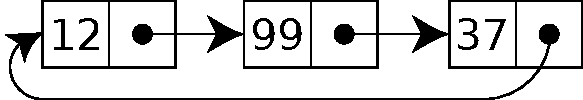
\includegraphics[width=.5\textwidth]{Circularly-linked-list} }
      \mode<article>{ 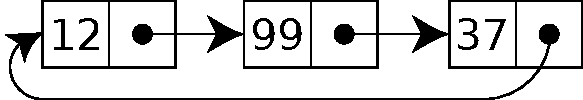
\includegraphics[width=.2\textwidth]{Circularly-linked-list} }
    \end{center}
  \end{block}
  \begin{block}{Doubly linked list}
    \begin{center}
      \mode<beamer>{ 
\includegraphics[width=.7\textwidth]{Doubly-linked-list} }
      \mode<article>{ 
\includegraphics[width=.3\textwidth]{Doubly-linked-list} }
    \end{center}
  \end{block}
\end{frame}

Linked lists are ill-suited for use cases where \emph{random access} is an important
operation. Instead, you use linked lists when \emph{iterating over the whole list} is
important and the \emph{dynamic addition and removal} of elements is
required. \citetitle[Sec.~6.1.3, \emph{Moving Through a Linked List}]{love2010linux}

See also: \citetitle{web:array-linkedlist}.

\begin{frame}{Circular doubly linked-lists}
  \begin{center}
    \mode<beamer>{ 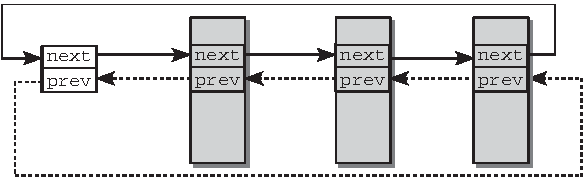
\includegraphics[width=\textwidth]{doubly-linked-list} }
    \mode<article>{ 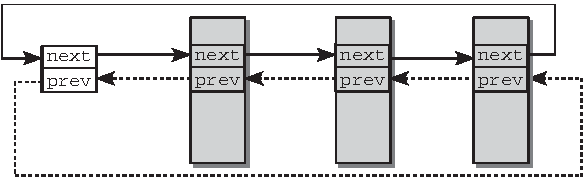
\includegraphics[width=.5\textwidth]{doubly-linked-list} }
  \end{center}
\end{frame}

See also: 
\begin{itemize}
\item \citetitle[Sec.~3.2.2.3, \emph{Doubly Linked Lists}]{bovet2005understanding};
\item \citetitle[Sec.~2.1, \emph{Common Kernel Data Types}]{rodriguez2005linux};
\item \citetitle{web:linkedlist};
\item \citetitle{web:klist}.
\end{itemize}

\begin{frame}[fragile=singleslide]
  \begin{block}{Things to note}
    \begin{enumerate}
    \item List is \emph{inside the data item} you want to link together.
    \item You \textbf{can put} ``\verb|struct list_head|'' \textbf{anywhere} in your structure.
    \item You \textbf{can name} ``\verb|struct list_head|'' \textbf{variable anything} you wish.
    \item You \textbf{can have} multiple lists!
    \end{enumerate}
  \end{block}
\end{frame}

\begin{frame}[fragile=singleslide]{Linked Lists}
  A linked list is initialized by using the \texttt{LIST\_HEAD} and
  \texttt{INIT\_LIST\_HEAD} macros
  \begin{block}{\texttt{include/linux/list.h}}%{\texttt{LIST\_HEAD} and \texttt{INIT\_ LIST\_HEAD}}
    \begin{center}
      \mode<beamer>{ 
\includegraphics[width=\textwidth]{list} }
      \mode<article>{ 
\includegraphics[width=.5\textwidth]{list} }      
    \end{center}
  \end{block}
  \begin{itemize}
  \item[Q1:] Why both \texttt{LIST\_HEAD\_INIT} and \texttt{INIT\_LIST\_HEAD}?
  \item[Q2:] Why \texttt{do-while}?
  \end{itemize}
\end{frame}

\paragraph{LIST\_HEAD}

When first encountering this, most people are confused because they have been taught to
implement linked lists by adding a pointer in a structure which points to the next similar
structure in the linked list. The drawback of this approach, and the reason for which the
kernel implements linked lists differently, is that you need to write code to handle
(adding/removing/etc) elements specifically for that data structure. Here, we can add a
struct \texttt{list\_head} field to any other data structure and, as we'll see shortly, make
it a part of a linked list. Moreover, if you want your data structure to be part of
several data structures, adding a few of these fields will work out just
fine\footnote{\url{http://kernelnewbies.org/FAQ/LinkedLists}}. \citetitle{kernelnewbies:faq/l72}

\subparagraph{Why is there a need to declare \texttt{LIST\_HEAD\_INIT} and
  \texttt{INIT\_LIST\_HEAD} they both seem to do the same thing?}

\begin{itemize}
\item An example \citetitle[Sec.~6.1.1, \emph{Defining a linked list}]{love2010linux}.
\item \texttt{LIST\_HEAD\_INIT} initializes one of these list head structure thingamajigs at
  compile time and so it doesn't actually generate any code, but stores constant values in
  a structure of which the address is known and
  fixed\footnote{\url{http://ubuntuforums.org/archive/index.php/t-1591281.html}}. \citetitle{ubuntuforums:linkl47}

  On the other hand, \texttt{INIT\_LIST\_HEAD} takes a pointer and so it could be a
  structure that is dynamically allocated, e.g. with ``\texttt{malloc}'' or one that is passed into
  your function... and then it does it's stuff at run time.
\item \texttt{LIST\_HEAD\_INIT} is a static initializer, \texttt{INIT\_LIST\_HEAD} is a
  function (in 2.6.11 it's still a macro). They both initialise a \texttt{list\_head} to be
  empty \footnote{\url{http://stackoverflow.com/questions/10262017/linux-kernel-list-list-head-init-vs-init-list-head}}. \citetitle{stackoverflow:c-lin84}

  If you are statically declaring a \texttt{list\_head}, you should use
  \texttt{LIST\_HEAD\_INIT}, e.g.:

  \begin{center}
\begin{ccode}
static struct list_head mylist = INIT_LIST_HEAD(mylist);
\end{ccode}
  \end{center}
  You should use \texttt{INIT\_LIST\_HEAD()} for a list head that is dynamically allocated,
  usually part of another structure. There are many examples in the kernel source.
\item \textbf{My understanding:} compile time list head initialization is better for
  kernel memory management e.g. slab allocation.
\item See also: \citetitle{wiki:malloc}
\end{itemize}

\begin{frame}{Example}
  \begin{center}
    \mode<beamer>{ 
\includegraphics[width=.5\textwidth]{fox-struct} }
    \mode<article>{ 
\includegraphics[width=.3\textwidth]{fox-struct} }
  \end{center}
  \begin{block}{The list needs to be initialized before in use}
    \begin{itemize}
    \item Run-time initialization
      \begin{center}
        \mode<beamer>{ 
\includegraphics[width=.8\textwidth]{fox-dynamic} }
        \mode<article>{ 
\includegraphics[width=.5\textwidth]{fox-dynamic} }
      \end{center}
    \item Compile-time initialization
      \begin{center}
        \mode<beamer>{ 
\includegraphics[width=.7\textwidth]{fox-static} }
        \mode<article>{ 
\includegraphics[width=.5\textwidth]{fox-static} }
      \end{center}
    \end{itemize}
  \end{block}
\end{frame}

See also:
\begin{itemize}
\item \citetitle[Sec.~6.1.4, \emph{The Linux Kernel's Implementation}]{love2010linux}
\item About \texttt{kmalloc()}, see \citetitle[Sec.~8.1, \emph{The Real Story of
    kmalloc}]{corbet05ldd}
\item \texttt{GFP MASK} \citetitle{web:pagealloc}
\end{itemize}

\begin{frame}
  \begin{block}{The \texttt{do while(0)} trick}
    \begin{center}
      \mode<beamer>{ 
\includegraphics[width=.7\textwidth]{macro} }
      \mode<article>{ 
\includegraphics[width=.5\textwidth]{macro} }
    \end{center}
  \end{block}
\end{frame}

\paragraph{do...while(0)}

\begin{center}
  
\includegraphics[width=.6\textwidth]{do-while}
\end{center}

See also:
\begin{itemize}
\item \citetitle{web:dowhile}
\item \citetitle{web:dowhile2}
\item \citetitle{web:dowhile3}
\end{itemize}
  
\begin{frame}[fragile=singleslide]
  \begin{block}{After \texttt{INIT\_LIST\_HEAD} macro is called}
    \begin{center}
      \mode<beamer>{ \mbox{
          \includegraphics[width=.25\textwidth]{list-head-2}\qquad
          
\includegraphics[width=.72\textwidth]{list} }}
      \mode<article>{ \mbox{
          \includegraphics[width=.2\textwidth]{list-head-2}\qquad
          
\includegraphics[width=.5\textwidth]{list} }}    
    \end{center}
  \end{block}
  Example: to start an empty \texttt{fox} list  
  \begin{center}
\begin{ccode}
static LIST_HEAD(fox_list);
\end{ccode}
  \end{center}
\end{frame}

\begin{frame}[fragile=singleslide]
  \begin{block}{Manipulating linked lists}
    \begin{itemize}
    \item To add a new member into \texttt{fox\_list}:
      \begin{itemize}
      \item[] \mintinline{c}{list_add(&new->list,&fox_list);}
        \begin{itemize}
        \item \mintinline{c}{fox_list->next->prev = new->list;}
        \item \mintinline{c}{new->list->next = fox_list->next;}
        \item \mintinline{c}{new->list->prev = fox_list;}
        \item \mintinline{c}{fox_list->next = new->list;}
        \end{itemize}
      \item[] \mintinline{c}{list_add_tail(&f->list,&fox_list);}
      \end{itemize}
    \item To remove an \mintinline{c}{old} node from list:
      \begin{itemize}
      \item[] \mintinline{c}{list_del(&old->list);}
        \begin{itemize}
        \item \mintinline{c}{old->list->next->prev = old->list->prev;}
        \item \mintinline{c}{old->list->prev->next = old->list->next;}
        \end{itemize}
      \end{itemize}
    \item a lot more...
    \end{itemize}
  \end{block}
\end{frame}

This function adds the new node to the given list immediately after the head node.

\begin{center}
  \mintinline{c}|list_add(struct list_head *new, struct list_head *head)|
\end{center}

Because the list is circular and generally has no concept of \emph{first} or \emph{last}
nodes, you can pass any element for \texttt{head}. If you do pass the ``\texttt{last}'' element,
however, this function can be used to implement a stack \citetitle[Sec.~6.1.5,
\emph{Manipulating Linked Lists}]{love2010linux}.

\begin{frame}[fragile=singleslide]{List Traversing}
  \begin{center}
\begin{ccode}
struct list_head *p;
list_for_each(p,fox_list){ ... }
\end{ccode}
  \end{center}
  \begin{block}{\texttt{list\_for\_each}}
    \begin{center}
      \mode<beamer>{ 
\includegraphics[width=\textwidth]{list2} }
      \mode<article>{ 
\includegraphics[width=.8\textwidth]{list2} }
    \end{center}
  \end{block}
  Not so useful. Usually we want the pointer to the container struct.
\end{frame}

\begin{frame}[fragile=singleslide]
  \begin{center}
    \mode<beamer>{ 
\includegraphics[width=.5\textwidth]{fox-struct} }
    \mode<article>{ 
\includegraphics[width=.3\textwidth]{fox-struct} }
  \end{center}
  \begin{itemize}
  \item[Q:] Given a pointer to \emph{\texttt{list}}, how to get a pointer to \emph{\texttt{fox}}?
    \begin{center}
      \mintinline{c}|f = list_entry(p, struct fox, list);|
    \end{center}
  \end{itemize}
  \begin{block}{\texttt{list\_entry(ptr, type, member)}}
    \begin{center}
      \mode<beamer>{ 
\includegraphics[width=\textwidth]{list-entry} }
      \mode<article>{ 
\includegraphics[width=.7\textwidth]{list-entry} }
    \end{center}
  \end{block}
\end{frame}

The code above deserves some explanation (Also read \citetitle{web:containerof}).

\begin{itemize}
\item \mintinline{c}{container_of(ptr,type,member)}: We have the address of the
  \mintinline{c}{struct list_head} field inside of another data structure (let's say
  \mintinline{c}{struct task_struct} for sake of example). The first line of the macro
  casts the value \texttt{0} into a pointer of the encapsulating data structure type
  (\mintinline{c}{struct task_struct} in our example). We use this pointer to access the
  field in that data structure which corresponds to our \verb|list_head| and get
  its type with the macro \texttt{typeof} to declare a pointer \texttt{mptr} initialized
  to the value contained in \texttt{ptr}. \citetitle{web:linkedlist}
\item How Does This Work? See \citetitle{web:klist}
\item \mintinline{c}{list_entry(ptr,type,member)}: \citetitle{web:klist2}
\end{itemize}

\begin{frame}{\texttt{list\_for\_each\_entry(pos, head, member)}}
  \begin{center}
    \mode<beamer>{ 
\includegraphics[width=\textwidth]{fox-lfee} }
    \mode<article>{ 
\includegraphics[width=.8\textwidth]{fox-lfee} }
  \end{center}
  \begin{block}{\texttt{list\_for\_each\_entry(pos, head, member)}}
    \begin{center}
      \mode<beamer>{ 
\includegraphics[width=\textwidth]{list-for-each-entry} }
      \mode<article>{ 
\includegraphics[width=.8\textwidth]{list-for-each-entry} }
    \end{center}
  \end{block}
\end{frame}

% \begin{frame}{Examples}{--- kernel/workqueue.c}
%   \begin{block}{The kernel adds \code{wq->list} to the system-wide list of work queues}
%     \begin{itemize}
%     \item[] \cfbox{red}{\code{list\_add(\&wq->list, \&workqueues);}}
%     \end{itemize}
%   \end{block}
%   \begin{block}{adds \code{work->entry} to the end of the list \code{cwq->worklist}}
%     \begin{itemize}
%     \item[] \cfbox{red}{\code{list\_add\_tail(\&work->entry, \&cwq->worklist);}}
%     \end{itemize}
%   \end{block}
%   \begin{block}{deleting an element from a list}
%     \begin{itemize}
%     \item[] \cfbox{red}{\code{list\_del(\&wq->list);}}
%     \end{itemize}
%   \end{block}
% \end{frame}

% \begin{itemize}
% \item \citetitle[Sec.~2.1.1]{rodriguez2005linux}.
% \item \citetitle[See.~sec 4.8, \emph{Work Queues},]{bovet2005understanding}
% \end{itemize}

\subsubsection{Queues}

Ref: \citetitle[Sec 6.2, \emph{Queues}]{love2010linux}

\begin{frame}{Queue (FIFO)}
  \begin{minipage}{.73\linewidth}
    \begin{block}{Circular buffer}
      \begin{description}
      \item[Empty:] $in == out$
      \item[Full:] $(in+1) \% BUFFER\_SIZE == out$
      \end{description}
    \end{block}
    Can be lock-free.
  \end{minipage}\hfill
  \begin{minipage}{.25\linewidth}
    \begin{center}
      \mode<beamer>{ 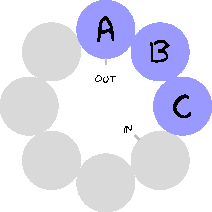
\includegraphics[width=\textwidth]{circular} }
      \mode<article>{ 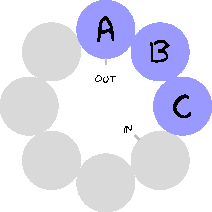
\includegraphics[width=\textwidth]{circular} }
    \end{center}
  \end{minipage}
\end{frame}

See also: \citetitle{wiki:circular-buf}

\begin{frame}{KFIFO}
  \begin{block}{\texttt{include/linux/kfifo.h}}
    \begin{center}
      \mode<beamer>{ 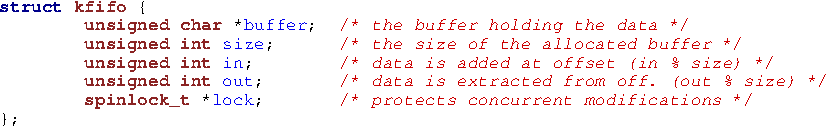
\includegraphics[width=\textwidth]{kfifo-struct} }
      \mode<article>{ 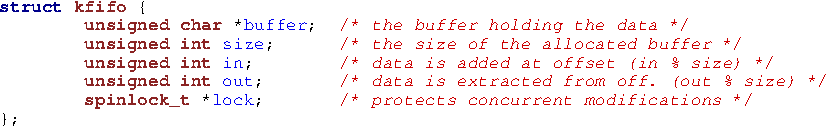
\includegraphics[width=.9\textwidth]{kfifo-struct} }
    \end{center}
  \end{block}
  The \emph{spinlock} is rarely needed.
\end{frame}

\begin{frame}
  Initialization:
  \mode<beamer>{
    \begin{itemize}
    \item[] 
\includegraphics[width=.7\textwidth]{kfifo-alloc}
    \item[] 
\includegraphics[width=.7\textwidth]{kfifo-init}
    \end{itemize} }
  \mode<article>{
    \begin{itemize}
    \item[] 
\includegraphics[width=.4\textwidth]{kfifo-alloc}
    \item[] 
\includegraphics[width=.4\textwidth]{kfifo-init}
    \end{itemize} }
  \begin{block}{Example: to have a \texttt{PAGE\_SIZE}-sized queue}
    \begin{center}
      \mode<beamer>{ 
\includegraphics[width=.8\textwidth]{kfifo-alloc2} }
      \mode<article>{ 
\includegraphics[width=.6\textwidth]{kfifo-alloc2} }
    \end{center}
  \end{block}
\end{frame}

See also: \citetitle[Sec.~6.2.2, \emph{Creating a queue}, p97]{love2010linux}

\begin{frame}{\texttt{kfifo} operations}
  \begin{center}
    \mode<beamer>{ 
\includegraphics[width=.95\textwidth]{kfifo-op} }
    \mode<article>{ 
\includegraphics[width=.7\textwidth]{kfifo-op} }
  \end{center}
\end{frame}

\begin{frame}{Example}
  \begin{enumerate}
  \item To enqueue 32 integers into \emph{\texttt{fifo}}
    \begin{center}
      \mode<beamer>{ 
\includegraphics[width=.6\textwidth]{kfifo-in} }
      \mode<article>{ 
\includegraphics[width=.4\textwidth]{kfifo-in} }
    \end{center}
  \item To dequeue and print all the items in the queue
    \begin{center}
      \mode<beamer>{ 
\includegraphics[width=.8\textwidth]{kfifo-out} }
      \mode<article>{ 
\includegraphics[width=.5\textwidth]{kfifo-out} }
    \end{center}
  \end{enumerate}
\end{frame}

\begin{itemize}
\item \mintinline{c}{kfifo_in()}: This function copies the \emph{\texttt{len}} bytes
  starting at \emph{\texttt{from}} into the queue represented by
  \emph{\texttt{fifo}}. \citetitle[Sec.~6.2.3 \emph{Enqueuing Data}, p98]{love2010linux}
  \begin{itemize}
  \item On success it returns the number of bytes enqueued.
  \item If less than \emph{\texttt{len}} bytes are free in the queue, the function copies
    only up to the amount of available bytes.Thus the return value can be less than
    \emph{\texttt{len}} or even zero, if nothing was copied.
  \end{itemize}
\item \mintinline{c}{kfifo_out()}: This function copies at most \emph{\texttt{len}} bytes
  from the queue pointed at by \emph{\texttt{fifo}} to the buffer pointed at by
  \emph{\texttt{to}}. \citetitle[Sec.~6.2.4, \emph{Dequeuing Data}, p98]{love2010linux}
  \begin{itemize}
  \item On success the function returns the number of bytes copied.
  \item If less than \emph{\texttt{len}} bytes are in the queue, the function copies less
    than requested.
  \end{itemize}
\end{itemize}

% \subsubsection{Maps}
% \label{sec:maps}

% \citetitle[Sec 6.3, \emph{Maps}]{love2010linux}

% \begin{frame}{Maps}
%   \begin{itemize}
%   \item Associative array
%   \item Implementation
%     \begin{itemize}
%     \item Hash tables
%     \item Binary search trees
%     \end{itemize}
%   \item Operations
%     \begin{itemize}
%     \item \code{add(key, value)}
%     \item \code{remove(key)}
%     \item \code{value = lookup(key)}
%     \end{itemize}
%   \end{itemize}
% \end{frame}

\subsubsection{Binary Trees}

Ref: \citetitle[Sec.~6.4, \emph{Binary Trees}]{love2010linux}

\begin{frame}{Trees}
  \begin{itemize}
  \item Used in Linux memory management
    \begin{itemize}
    \item fast store/retrieve a single piece of data among many
    \end{itemize}
  \item generally implemented as \emph{linked lists} or \emph{arrays}
  \item the process of moving through a tree --- \emph{traversing}
  \end{itemize}
\end{frame}

\begin{frame}{Binary Search Tree}
  \begin{center}
    \includegraphics[width=.2\textwidth]{Binary_search_tree}
  \end{center}
  \begin{block}{Properties:}
    \begin{itemize}
    \item The left subtree of a node contains only nodes with keys less than the node's
      key.
    \item The right subtree of a node contains only nodes with keys greater than the
      node's key.
    \item Both the left and right subtrees must also be binary search trees.
    \end{itemize}
  \end{block}
  Efficient in:
  \begin{enumerate}
  \item searching for a given node
  \item in-order traversal (e.g. Left-Root-Right)
  \end{enumerate}
\end{frame}

See also:
\begin{itemize}
\item \citetitle{wiki:bin-search-tree}
\item \url{http://www.cs.duke.edu/~reif/courses/alglectures/skiena.lectures/lecture8.pdf}
\item \url{http://www.cse.iitk.ac.in/users/sbaswana/Courses/ESO211/bst.pdf/}
\item \url{http://www.personal.kent.edu/~rmuhamma/Algorithms/MyAlgorithms/binarySearchTree.htm}
\end{itemize}

\begin{frame}<beamer>
    \begin{tabular}{cc}
      Unbalanced binary tree&Balanced binary tree\\
      \includegraphics[width=.3\textwidth]{Unbalanced_binary_tree}&
      \includegraphics[width=.4\textwidth]{AVLtreef}\\
      &\\
      \multicolumn2{c}{Red-black tree}\\
      \multicolumn2{c}{\includegraphics[width=.6\textwidth]{Red-black-tree}}\\
    \end{tabular}
\end{frame}

\begin{figure}[!ht]
  \centering
  \begin{minipage}[b]{.2\linewidth}
    \includegraphics[width=\textwidth]{Unbalanced_binary_tree}
    \caption{Unbalanced binary tree}
  \end{minipage}\quad
  \begin{minipage}[b]{.3\linewidth}
    \includegraphics[width=\textwidth]{AVLtreef}
    \caption{Balanced binary tree}
  \end{minipage}\quad
  \begin{minipage}[b]{.3\linewidth}
    \includegraphics[width=\textwidth]{Red-black-tree}
    \caption{Red-black tree}
  \end{minipage}
\end{figure}

\begin{itemize}
\item A \emph{balanced binary search tree} is a binary search tree in which the depth of
  all leaves differs by at most one.
\item A \emph{self-balancing binary search tree} is a binary search tree that attempts, as
  part of its normal operations,to remain (semi) balanced.
\end{itemize}

See also:
\begin{itemize}
\item \citetitle{wiki:tree}
\item \citetitle{wiki:bin-tree}
\item \citetitle{wiki:bin-search-tree}
\item \citetitle{wiki:avl-tree}
\item \citetitle{wiki:rbtree}
\item \citetitle{wiki:big-o}
\end{itemize}

\begin{frame}
  \mode<beamer>{
    \begin{center}
      \includegraphics[width=.2\textwidth]{Red-black-tree}
    \end{center} }
  \begin{description}
  \item[Red-black tree] A type of \emph{self-balancing BST} in which each node has a red
    or black color attribute.
  \end{description}  
  \begin{block}{Properties to make it \emph{semi-balanced}:}
    \begin{enumerate}
    \item All nodes are either red or black
    \item Leaf nodes are black (root's color)
    \item Leaf nodes do not contain data (NULL)
    \item All non-leaf nodes have two children
    \item If a node is red, both its children are black
    \item When traversing from the root node to a leaf, each path contains the same number
      of black nodes
      % \item $O(log(n))$
    \end{enumerate}
    These properties ensure that \emph{the deepest leaf has a depth of no more than double that
    of the shallowest leaf}.
  \end{block}
\end{frame}

\begin{itemize}
\item Property 5 implies that on any path from the root to a leaf, red nodes must not be
  adjacent.  However, any number of black nodes may appear in a sequence.
\item Taken together, these properties ensure that the deepest leaf has a depth of no more
  than double that of the shallowest leaf. Consequently, the tree is always
  semi-balanced. Why this is true is surprisingly simple. First, by property five, a red
  node cannot be the child or parent of another red node. By property six, all paths
  through the tree to its leaves have the same number of black nodes.The longest path
  through the tree alternates red and black nodes.Thus the shortest path, which must have
  the same number of black nodes, contains only black nodes.Therefore, the longest path
  from the root to a leaf is no more than double the shortest path from the root to any
  other leaf. \citetitle[p105]{love2010linux}
\item \href{http://www.cs.auckland.ac.nz/\char`~jmor159/PLDS210/red\_black.html}{\emph{Data
      structure and algorithms, Sec 8.2, Red-black
      tree}}\footnote{\url{http://www.cs.auckland.ac.nz/~jmor159/PLDS210/red_black.html}}
\item \href{http://www.ece.uc.edu/\char`~franco/C321/html/RedBlack/redblack.html}{Red-black tree
    Java applet demo}
  \footnote{\url{http://www.ece.uc.edu/~franco/C321/html/RedBlack/redblack.html}}
\end{itemize}

\begin{frame}
  \begin{block}{Advantages}
    \begin{itemize}
    \item faster real-time bounded worst case performance for insertion and deletion
      \begin{itemize}
      \item usually at most two rotations% and three rotations, respectively, to balance the tree
      \end{itemize}
    \item slightly slower (but still $O(log n)$) lookup time
    \end{itemize}
  \end{block}
  \begin{block}{Many red-black trees in use in the kernel}
    \begin{itemize}
    \item The deadline and CFQ I/O schedulers employ rbtrees to track requests;
    \item the packet CD/DVD driver does the same
    \item The high-resolution timer code uses an rbtree to organize outstanding timer
      requests
    \item The ext3 filesystem tracks directory entries in a red-black tree
    \item Virtual memory areas (VMAs) are tracked with red-black trees
    \item epoll file descriptors, cryptographic keys, and network packets in the
      ``hierarchical token bucket'' scheduler
    \end{itemize}
  \end{block}
\end{frame}

See also:
\begin{itemize}
\item \citetitle{web:rbtree}
\item \citetitle{web:rbtree2}
\end{itemize}

\begin{frame}[fragile=singleslide]
  \begin{block}{\texttt{<linux/rbtree.h>}}
    \begin{center}
      \mode<beamer>{ \includegraphics[width=.75\textwidth]{rbtree} }
      \mode<article>{ \includegraphics[width=.4\textwidth]{rbtree} }
    \end{center}
  \end{block}
  To create a new empty tree:
  \begin{center}
    \mintinline{c}{struct rb_root root = RB_ROOT;}
  \end{center}
\end{frame}

\begin{itemize}
\item \href{http://www.kerneltravel.net/jiaoliu/kern-rbtree.html}{Linux内核中的红黑树}\footnote{\url{http://www.kerneltravel.net/jiaoliu/kern-rbtree.html}}
\item ``\mintinline{c}{(struct rb_root){ NULL, }}'' is a compound literal
  \citetitle[Sec.~6.26]{web:gcc}. ``\mintinline{c}{{ NULL, }}'' is an \emph{initializer
    list} \citetitle[Sec.~6.7.8, p125, \emph{Initialization}]{iso:c99}. It initializes the
  1\textsuperscript{st} element (a pointer) to \emph{\texttt{NULL}}, and initializes the rest
  (omitted) as if they are static objects: arithmetic types are initialized to \emph{\texttt{0}};
  pointers are initialized to \emph{\texttt{NULL}} \citetitle{web:ibm-c}.

  See also:
  \begin{itemize}
  \item \citetitle[Sec.~6.5.2.5, p75, \emph{Compound literals}]{iso:c99}
  \item \citetitle[Sec.~6.27, \emph{Designated Initializers}]{iso:c99}
  \end{itemize}
\end{itemize}

\begin{frame}{Example}
  \begin{center}
    \mode<beamer>{ \includegraphics[width=.4\textwidth]{fox-rbtree} }
    \mode<article>{ \includegraphics[width=.3\textwidth]{fox-rbtree} }
  \end{center}
  \begin{block}{Search}
    \begin{center}
      \mode<beamer>{ \includegraphics[width=\textwidth]{fox-search} }
      \mode<article>{ \includegraphics[width=.7\textwidth]{fox-search} }
    \end{center}
  \end{block}
\end{frame}

\begin{frame}{Example}
  \begin{block}{Searching for a specific page in the page cache}
    \begin{center}
      \mode<beamer>{ \includegraphics[width=\textwidth]{rb-search} }
      \mode<article>{ \includegraphics[width=.7\textwidth]{rb-search} }
    \end{center}
  \end{block}
\end{frame}

See also:
\begin{itemize}
\item \texttt{include/linux/rbtree.h}  
\item \citetitle[p106-107]{love2010linux}
\item \citetitle[Sec.~9.3, \emph{Memory Regions}]{bovet2005understanding}
\end{itemize}

\subsection{Assembly}

\begin{frame}{x86 Assembly}
  \begin{block}{The Pentium class x86 architecture}
    \begin{itemize}
    \item Data ordering is in Little Endian
    \item Memory access is in byte (8 bit), word (16 bit), double word (32 bit), and quad
      word (64 bit).
    \item the usual registers for code and data instructions can be broken down into three
      categories: \emph{control}, \emph{arithmetic}, and \emph{data}.
    \end{itemize}
  \end{block}
\end{frame}

\begin{frame}
  \begin{block}{Byte ordering is architecture dependent}
    Storing an int (\texttt{0x01234567}) at address \texttt{0x100}:
    \begin{center}
      \mode<beamer>{ \includegraphics[width=.7\textwidth]{endian} }
      \mode<article>{ \includegraphics[width=.5\textwidth]{endian} }
    \end{center}
  \end{block}
\end{frame}

See also: \citetitle{wiki:endianness}

\begin{frame}
  \begin{center}
    \mode<beamer>{ \includegraphics[width=.7\textwidth]{registers}}
    \mode<article>{ \includegraphics[width=.5\textwidth]{registers}}
  \end{center}
  \begin{block}{Three kinds of registers}
    \begin{enumerate}
    \item general purpose registers
    \item segment registers
    \item status/control registers
    \end{enumerate}
  \end{block}
\end{frame}

\begin{frame}
  \begin{block}{General purpose registers}
    \begin{multicols}{2}
      \begin{description}
      \item[EAX] \uline{A}ccumulator register
      \item[EBX] \uline{B}ase register
      \item[ECX] \uline{C}ounter for loop operations
      \item[EDX] \uline{D}ata register
        \columnbreak
      \item[ESI] \uline{S}ource \uline{I}ndex
      \item[EDI] \uline{D}estination \uline{I}ndex
      \item[ESP] \uline{S}tack \uline{P}ointer
      \item[EBP] \uline{B}ase \uline{P}ointer pointing to the top of previous stack frame
      \end{description}
    \end{multicols}
  \end{block}
\end{frame}

The eight general-purpose registers in the x86 processor family each have an unique
purpose. Each register has special instructions and opcodes which make fulfilling this
purpose more convenient or efficient. \citetitle{web:thear30}

\begin{description}
\item[EAX] There are three major processor architectures: register, stack, and
  accumulator. In a register architecture, operations such as addition or subtraction can
  occur between any two arbitrary registers. In a stack architecture, operations occur
  between the top of the stack and other items on the stack. In an accumulator
  architecture, the processor has single calculation register called the accumulator. All
  calculations occur in the accumulator, and the other registers act as simple data
  storage locations.

  The x86 processor does not have an accumulator architecture. It does, however, have an
  accumulator-like register: \texttt{EAX/AL}. Although most calculations can occur between
  any two registers, the instruction set gives the accumulator special preference as a
  calculation register.

  Since most calculations occur in the accumulator, the x86 architecture contains many
  optimized instructions for moving data in and out of this register. ... In your code,
  try to perform as much work in the accumulator as possible. As you will see, the
  remaining seven general-purpose registers exist primarily to support the calculation
  occurring in the accumulator.
\item[EBX] The base register gets its name from the \texttt{XLAT}
  instruction. \texttt{XLAT} looks up a value in a table using \texttt{AL} as the index
  and \texttt{EBX} as the base. \texttt{XLAT} is equivalent to
  \mintinline{nasm}{MOV AL, [BX+AL]},
  which is sometimes useful if you need to replace one 8-bit value with another from a
  table (Think of color look-up).

  So, of all the general-purpose registers, \texttt{EBX} is the only register without an
  important dedicated purpose. It is a good place to store an extra pointer or calculation
  step, but not much more.
\item[EDX] Of the seven remaining general-purpose registers, the data register,
  \texttt{EDX}, is most closely tied to the accumulator. Instructions that deal with over
  sized data items, such as multiplication, division, \texttt{CWD}, and \texttt{CDQ}, store the most
  significant bits in the data register and the least significant bits in the
  accumulator. In a sense, the data register is the 64-bit extension of the
  accumulator. The data register also plays a part in I/O instructions. In this case, the
  accumulator holds the data to read or write from the port, and the data register holds
  the port address.
\item[ECX] The count register, \texttt{ECX}, is the x86 equivalent of the ubiquitous
  variable \texttt{i}. Every counting-related instruction in the x86 uses \texttt{ECX}. The most
  obvious counting instructions are \texttt{LOOP}, \texttt{LOOPZ}, and \texttt{LOOPNZ}. Another
  counter-based instruction is \texttt{JCXZ}, which, as the name implies, jumps when the
  counter is 0. The count register also appears in some bit-shift operations, where it
  holds the number of shifts to perform. Finally, the count register controls the string
  instructions through the \texttt{REP}, \texttt{REPE}, and \texttt{REPNE} prefixes. In this
  case, the count register determines the maximum number of times the operation will
  repeat.

  Particularly in demos, most calculations occur in a loop. In these situations,
  \texttt{ECX} is the logical choice for the loop counter, since no other register has so
  many branching operations built around it. The only problem is that this register counts
  downward instead of up as in high level languages. Designing a downward-counting is not
  hard, however, so this is only a minor difficulty.
\item[EDI] Every loop that generates data must store the result in memory, and doing so
  requires a moving pointer. The destination index, EDI, is that pointer. The destination
  index holds the implied write address of all string operations. The most useful string
  instruction, remarkably enough, is the seldom-used \texttt{STOS}. \texttt{STOS} copies
  data from the accumulator into memory and increments the destination index. This
  one-byte instruction is perfect, since the final result of any calculation should be in
  the accumulator anyhow, and storing results in a moving memory address is a common task.

  See also: \citetitle{stack:stos}
\item[ESI] The source index, \texttt{ESI}, has the same properties as the destination
  index. The only difference is that the source index is for reading instead of
  writing. Although all data-processing routines write, not all read, so the source index
  is not as universally useful. When the time comes to use it, however, the source index
  is just as powerful as the destination index, and has the same type of instructions.

  In situations where your code does not read any sort of data, of course, using the
  source index for convenient storage space is acceptable.
\item[ESP \& EBP] When a block of code calls a function, it pushes the
  parameters and the return address on the stack. Once inside, function sets the base
  pointer equal to the stack pointer and then places its own internal variables on the
  stack. From that point on, the function refers to its parameters and variables relative
  to the base pointer rather than the stack pointer. Why not the stack pointer?  For some
  reason, the stack pointer lousy addressing modes. In 16-bit mode, it cannot be a
  square-bracket memory offset at all. In 32-bit mode, it can be appear in square brackets
  only by adding an expensive SIB byte to the opcode.

  In your code, there is never a reason to use the stack pointer for anything other than
  the stack. The base pointer, however, is up for grabs. If your routines pass parameters
  by register instead of by stack (they should), there is no reason to copy the stack
  pointer into the base pointer. The base pointer becomes a free register for whatever you
  need.
\end{description}

\begin{frame}
  \begin{block}{Segment registers}
    \begin{description}
    \item[CS] Code segment
    \item[SS] Stack segment
    \item[DS,ES,FS,GS] Data segment
    \end{description}
  \end{block}
  \begin{block}{A memory address is an offset in a segment}
    \begin{description}
    \item[ES:EDI] references memory in the ES (extra segment) with an offset of the value in the EDI
    \item[DS:ESI]
    \item[CS:EIP]
    \item[SS:ESP] 
    \end{description}
  \end{block}
\end{frame}

\begin{frame}
  \begin{block}{State/Control registers}
    \begin{description}
    \item[EFLAGS] Status, control, and system flags
    \item[EIP] The instruction pointer, contains an offset from CS (CS:EIP)
    \end{description}
  \end{block}
  \begin{block}{FLAGS}
    \begin{tabular}{|l|l|l|l|l|l|l|l|l|l|l|l|l|l|l|l|}
      \hline
      15&&&&11&&&&7&6&&&&&&0\\\hline
      -&-&-&-&O&D&I&T&S&Z&-&A&-&P&-&C\\\hline
    \end{tabular}
    \begin{multicols}{2}
      \begin{description}
      \item[CF] Carry flag
      \item[ZF] Zero flag
      \item[SF] Sign flag, Negative flag
      \item[OF] Overflow flag
      \end{description}
    \end{multicols}
  \end{block}
\end{frame}

See also: \citetitle{wiki:eflags}

\begin{frame}
  \begin{block}{Control Instructions \scriptsize{(Intel syntax)}}
    \begin{small}{\ttfamily
      \begin{tabular}{lll}
        \textbf{Instruction}&\textbf{Function}&\textbf{EFLAGS}\\\hline
        je&Jump if equal&$ZF=1$\\
        jg&Jump if greater&$ZF=0$\\
        &&$SF=OF$\\
        jge&Jump if greater or equal&$SF=OF$\\
        jl&Jump if less&$SF\ne{}OF$\\
        jle&Jump if less or equal&$ZF=1$\\
        jmp&Unconditional jump&unconditional
      \end{tabular}}
    \end{small}
  \end{block}
  \begin{block}{Example \scriptsize{(Intel syntax)}}
    \begin{center}
      \mode<beamer>{ \includegraphics[width=\textwidth]{asm2} }
      \mode<article>{ \includegraphics[width=.5\textwidth]{asm2} }
    \end{center}
  \end{block}
\end{frame}

\begin{frame}[fragile=singleslide]
  Data can be moved
  \begin{itemize}
  \item between registers
  \item between registers and memory
  \item from a constant to a register or memory, but
  \item \textbf{NOT} from one memory location to another
  \end{itemize}
  \begin{block}{Data instructions \scriptsize{(Intel syntax)}}
    \begin{enumerate}
    \item \mintinline{nasm}{mov eax, ebx}
      \begin{itemize}
      \item[] Move 32 bits of data from \texttt{ebx} to \texttt{eax}
      \end{itemize}
    \item \mintinline{nasm}{mov eax, WORD PTR[data3]}
      \begin{itemize}
      \item[] Move 32 bits of data from memory variable \texttt{data3} to \texttt{eax}
      \end{itemize}
    \item \mintinline{nasm}{mov BYTE PTR[char1], al}
      \begin{itemize}
      \item[] Move 8 bits of data from \texttt{al} to memory variable \texttt{char1}
      \end{itemize}
    \item \mintinline{nasm}{mov eax, 0xbeef}
      \begin{itemize}
      \item[] Move the constant value \texttt{0xbeef} to \texttt{eax}
      \end{itemize}
    \item \mintinline{nasm}{mov WORD PTR[my_data], 0xbeef}
      \begin{itemize}
      \item[] Move the constant value \texttt{0xbeef} to the memory variable
          \texttt{my\_data}
      \end{itemize}
    \end{enumerate}
  \end{block}
\end{frame}

\begin{frame}[fragile=singleslide]
  \begin{block}{Address operand syntax \scriptsize{(AT\&T syntax)}}
    \begin{center}
      \mintinline{gas}{ADDRESS_OR_OFFSET(%BASE_OR_OFFSET, %INDEX, MULTIPLIER)}
    \end{center}
    \begin{itemize}
    \item up to 4 parameters
      \begin{itemize}
      \item \texttt{ADDRESS\_OR\_OFFSET} and \texttt{MULTIPLIER} must be
          \textbf{constants}
      \item \texttt{\%BASE\_OR\_OFFSET} and \texttt{\%INDEX} must be
          \textbf{registers}
      \end{itemize}
    \item all of the fields are optional
      \begin{itemize}
      \item if any of the pieces is left out, substituted it with zero
      \end{itemize}
    \item final address =
      \begin{itemize}
      \item[] \scriptsize{\texttt{ADDRESS\_OR\_OFFSET + \%BASE\_OR\_OFFSET + \%INDEX * MULTIPLIER}}
      \end{itemize}
    \end{itemize}
  \end{block}
\end{frame}

\begin{frame}[fragile=singleslide]
  \begin{block}{Why so complicate?}
    To serve several \emph{addressing modes}
    \begin{description}
    \item[direct addressing mode] \mintinline{gas}{movl ADDRESS, %eax}
      \begin{itemize}
      \item load data at \texttt{ADDRESS} into \texttt{\%eax}
      \end{itemize}
    \item[indexed addressing mode] \mintinline{gas}{movl START(,%ecx,1), %eax}
        \begin{itemize}
        \item[-] \texttt{START} -- starting address;\qquad - \texttt{\%ecx} -- offset/index
        \end{itemize}
    \item[indirect addressing mode] \mintinline{gas}{movl (%eax), %ebx}
      \begin{itemize}
      \item load data at address pointed by \texttt{\%eax} into \texttt{\%ebx}
      \item \texttt{\%eax} contents an address pointer
      \end{itemize}
    \item[base pointer addressing mode] \mintinline{gas}{movl 4(%eax), %ebx}
    \end{description}
  \end{block}
  \begin{description}
  \item[immediate mode] \mintinline{gas}|movl $12, %eax|%$
    \begin{itemize}
    \item[without \texttt{\$}] Direct addressing
    \end{itemize}
  \end{description}
\end{frame}

\begin{frame}[fragile=singleslide]
  \begin{minipage}{.65\linewidth}
    \begin{block}{indexed addressing mode}
      \begin{center}
        \mintinline{gas}{movl START(,%ecx,1), %eax}
      \end{center}
      \begin{description}
      \item[\texttt{START}] starting address
      \item[\texttt{\%ecx}] offset/index
      \end{description}
    \end{block}
    \begin{block}{\mintinline{gas}{START(,INDEX,MULTIPLIER)}:}
      \begin{itemize}
      \item to access the 4\textsuperscript{th} byte from location \texttt{2002}
        \begin{itemize}
        \item[] $2002(,3,1) = 2002+3\times{}1 = 2005$
        \end{itemize}
      \item to access the 4\textsuperscript{th} word from location \texttt{2002}
        \begin{itemize}
        \item[] $2002(,3,4)= 2002+3\times{}4 = 2014$
        \end{itemize}
      \end{itemize}
    \end{block}
  \end{minipage}\hfill
  \begin{minipage}{.29\linewidth}
    \begin{center}
      \mode<beamer>{ \includegraphics[width=\textwidth]{indexed-addressing} }
      \mode<article>{ \includegraphics[width=.5\textwidth]{indexed-addressing} }
    \end{center}
  \end{minipage}
\end{frame}

In \emph{indexed addressing mode}, if you have a set of numbers starting at location
\texttt{2002}, you can cycle between each of them using an index register.

The \emph{multiplier} allows you to access memory a byte at a time or a word at a time (4
bytes).

\begin{itemize}
\item[e.g.] If you are accessing an entire word, your index will need to be multiplied by
  4 to get the exact location of the fourth element from your address.

  For example, if you wanted to access the fourth byte from location \texttt{2002}, you
  would load your index register with \texttt{3} (remember, we start counting at
  \texttt{0}) and set the multiplier to \texttt{1} since you are going a byte at a
  time. This would get you location \texttt{2005}. However, if you wanted to access the
  fourth word from location \texttt{2002}, you would load your index register with
  \texttt{3} and set the multiplier to \texttt{4}. This would load from location
  \texttt{2014} - the fourth word. Take the time to calculate these yourself to make sure
  you understand how it works.
\end{itemize}

See also: \citetitle[Sec.~2.5, \emph{Data Accessing Methods}]{bartlett2009programming}

\begin{frame}
  \begin{block}{Example \scriptsize{(AT\&T syntax)}}
    \begin{center}
      \mode<article>{ \includegraphics[width=.5\textwidth]{asm3} }
      \mode<beamer>{ \includegraphics[width=.6\textwidth]{asm3} }
    \end{center}
  \end{block}
  \begin{itemize}
  \item each word is 4 bytes long
  \item stack grows downward
  \item \texttt{mov\uline{l}} --- long, 32 bits
  \item \texttt{\%\uline{e}ax} --- extended, 32 bits
  \end{itemize}
\end{frame}

\begin{itemize}
\item \texttt{4(\%esp)} --- base pointer addressing mode.
  \begin{center}
    \texttt{4(\%esp) = 4(\%esp, , ) = 4 + \%esp + 0*0}
  \end{center}
\end{itemize}

\begin{frame}
  \begin{block}{Example \scriptsize{(AT\&T syntax)}}
    \mode<beamer>{ \includegraphics[width=\textwidth]{asm} }
    \mode<article>{ \includegraphics[width=.5\textwidth]{asm} }
    % \cfbox{red}{\code{movl -4(\%ebp, \%edx, 4), \%eax}}
    %     \begin{itemize}
    %     \item {\scriptsize{load \code{*(ebp - 4 + (edx * 4))} into \code{eax}}}
    %     \end{itemize}
  \end{block}
\end{frame}

\begin{itemize}
\item \emph{GAS Syntax} \citetitle{wikibooks-gas}.
\item \citetitle[Sec.~3.5, \emph{Addressing Modes}]{bartlett2009programming}
\item \texttt{movl} --- Data operation. load data into somewhere(register/memory).
\item \texttt{leal} --- Address operation. load effective address. \citetitle[Appendix.~B,
  p259]{bartlett2009programming}.
\end{itemize}

\begin{frame}
  \begin{block}{Example --- stack setup \scriptsize{(AT\&T syntax)}}
      \begin{center}
        \mode<article>{ \includegraphics[width=.6\textwidth]{asm4} }
        \mode<beamer>{ \includegraphics[width=\textwidth]{asm4} }
      \end{center}
  \end{block}
\end{frame}

\subsubsection{Assembly Language Examples}

\begin{frame}{Stack Setup}
  \begin{block}{Before executing a function, the program}
    \begin{itemize}
    \item pushes all of the parameters for the function onto the stack. Then
    \item issues a \emph{call} instruction indicating which function it wishes
      to start. The call instruction does two things
      \begin{enumerate}
      \item pushes the address of the next instruction (return address) onto the
        stack.
      \item modifies the instruction pointer (\texttt{\%eip}) to point to the start
        of the function.
      \end{enumerate}
    \end{itemize}
  \end{block}
\end{frame}

See also: \citetitle[Sec.~4.3, \emph{Assembly-Language Functions using the C Calling
    Convention}, p54]{bartlett2009programming}.

\begin{frame}[fragile=singleslide]
  \begin{block}{At the time the function starts...}
    The stack looks like this:
    \begin{small}
\begin{verbatim}
          Parameter #N
          ...
          Parameter 2
          Parameter 1
          Return Address <- (%esp)
\end{verbatim}
    \end{small}
  \end{block}
\end{frame}

\begin{frame}[fragile=singleslide]
  \begin{block}{The function initializes the \texttt{\%ebp}}
    \begin{small}
\begin{verbatim}
        pushl %ebp
        movl %esp, %ebp
\end{verbatim}
    \end{small}
    Now the stack looks like this:
    \begin{small}
\begin{verbatim}
        Parameter #N <- N*4+4(%ebp)
        ...
        Parameter 2 <- 12(%ebp)
        Parameter 1 <- 8(%ebp)
        Return Address <- 4(%ebp)
        Old %ebp <- (%esp) and (%ebp)
\end{verbatim}
    \end{small}
\end{block}
  each parameter can be accessed using base pointer addressing mode using the \texttt{\%ebp}
  register
\end{frame}

\begin{frame}[fragile=singleslide]%{Stack Setup}
  \begin{block}{The function reserves space for locals}
    \begin{center}
      \mintinline{gas}{subl $8, %esp}%$
    \end{center}
    Our stack now looks like this:
    \begin{small}
\begin{verbatim}
        Parameter #N <- N*4+4(%ebp)
        ...
        Parameter 2 <- 12(%ebp)
        Parameter 1 <- 8(%ebp)
        Return Address <- 4(%ebp)
        Old %ebp <- (%ebp)
        Local Variable 1 <- -4(%ebp)
        Local Variable 2 <- -8(%ebp) and (%esp)
\end{verbatim}
    \end{small}
\end{block}
\end{frame}

\begin{frame}[fragile=singleslide]
  \begin{block}{When a function is done executing, it does three things:}
    \begin{enumerate}
    \item stores its return value in \texttt{\%eax}
    \item resets the stack to what it was when it was called
    \item \texttt{ret} --- \mintinline{gas}{popl %eip}
        \#set \texttt{eip} to \emph{return address}
        % returns control back to wherever it was called from % This is done
        % using the ret instruction, which pops whatever value is at the top of the stack,
        % and
        % sets the instruction pointer, %eip, to that value.
    \end{enumerate}
  \end{block}
  \begin{center}
\begin{gascode}
        movl %ebp, %esp
        popl %ebp
        ret
\end{gascode}
  \end{center}
\end{frame}

\begin{frame}[fragile=singleslide]
  \begin{block}{After \texttt{ret}}
    \begin{small}
\begin{verbatim}
        Parameter #N
        ...
        Parameter 2
        Parameter 1 <- (%esp)
\end{verbatim}
  \end{small}
\end{block}
  \begin{block}{How about the \texttt{parameters}?}
    \begin{itemize}
    \item Under many calling conventions the items popped off the stack by the epilogue
      include the original argument values, in which case there usually are no further
      stack manipulations that need to be done by the caller.
    \item With some calling conventions, however, it is the caller's responsibility to
      remove the arguments from the stack after the return.
    \end{itemize}
  \end{block}
\end{frame}

The calling code also needs to pop off all of the parameters it pushed onto the stack in
order to get the stack pointer back where it was (you can also simply add \texttt{4 × number
  of paramters} to \texttt{\%esp} using the \texttt{addl} instruction, if you don't need the
values of the parameters anymore). \citetitle[p58]{bartlett2009programming}

See also: \citetitle[Sec.~4.3, \emph{Return processing}]{wiki:callstack}

\begin{frame}{Generating Assembly From C Code}
  \begin{minipage}{.22\linewidth}
    \begin{block}{\texttt{simple.c}}
      \begin{center}
        \mode<beamer>{ \includegraphics[width=.8\textwidth]{simpleC} }
        \mode<article>{ \includegraphics[width=.5\textwidth]{simpleC} }
      \end{center}
    \end{block}
    \begin{small}
      \begin{itemize}
      \item[\$] \texttt{gcc -S simple.c}
      \end{itemize}
    \end{small}
  \end{minipage}\qquad
  \begin{minipage}{.7\linewidth}
    \begin{block}{\texttt{simple.s} \scriptsize{(AT\&T syntax)}}
      \begin{center}
        \mode<article>{ \includegraphics[width=.7\textwidth]{simpleS} }
        \mode<beamer>{ \includegraphics[width=\textwidth]{simpleS} }
      \end{center}
    \end{block}
  \end{minipage}
\end{frame}

See also:
\begin{itemize}
\item[\$] \mintinline{sh}{info gas 'Pseudo Ops'}
\item \href{http://stackoverflow.com/questions/3564752/what-is-cfi-and-lfe-in-assembly-code-produced-by-gcc-from-c-program}{\emph{What
      is \texttt{.cfi} and \texttt{.LFE} in assembly code produced by GCC from c++ program?}}
  \footnote{\url{http://stackoverflow.com/questions/3564752/what-is-cfi-and-lfe-in-assembly-code-produced-by-gcc-from-c-program}}
  \begin{itemize}
  \item \texttt{.LFB} --- Local Function Begin
  \item \texttt{.LFE} --- Local Function End
  \end{itemize}
\item \href{http://stackoverflow.com/questions/7534420/gas-explanation-of-cfi-def-cfa-offset}{\emph{GAS: Explanation of \texttt{.cfi\_def\_cfa\_offset}}}
  \footnote{\url{http://stackoverflow.com/questions/7534420/gas-explanation-of-cfi-def-cfa-offset}}
\item \href{http://stackoverflow.com/questions/8478491/understanding-base-pointer-and-stack-pointers-in-context-with-gcc-output}{\emph{Understanding gcc generated assembly}}
  \footnote{\url{http://stackoverflow.com/questions/8478491/understanding-base-pointer-and-stack-pointers-in-context-with-gcc-output}}
\item \href{http://sourceware.org/binutils/docs/as/Pseudo-Ops.html\#Pseudo-Ops}{\emph{Assembler
    directives}}\footnote{\url{http://sourceware.org/binutils/docs/as/Pseudo-Ops.html\#Pseudo-Ops}}
\item \href{http://blog.mozilla.com/respindola/2011/05/12/cfi-directives/}{\emph{cfi directives}}
  \footnote{\url{http://blog.mozilla.com/respindola/2011/05/12/cfi-directives/}}
\end{itemize}

\begin{frame}{Outline of an Assembly Language Program}
  \begin{block}{Assembler directives (Pseudo-Ops)}
    Anything starting with a `\texttt{.}'
    \begin{description}
    \item[\texttt{.section .data}] starts the data section
    \item[\texttt{.section .text}] starts the text section
    \item[\texttt{.globl SYMBOL}] \ 
      \begin{itemize}
      \item[\texttt{SYMBOL}] is a \emph{symbol} marking the location of a program
      \item[\texttt{.globl}] makes the symbol visible to `\texttt{ld}'
      \end{itemize}
    \item[\texttt{LABEL:}] a \emph{label} defines a \emph{symbol}'s value (address)
    \end{description}
  \end{block}
\end{frame}

\begin{frame}{Generating Assembly From C Code}
  \begin{minipage}{.35\linewidth}
    \begin{block}{\texttt{simple.s} \scriptsize{(Oversimplified)}}
      \begin{center}
        \mode<beamer>{ \includegraphics[width=.9\textwidth]{simple2S} }
        \mode<article>{ \includegraphics[width=.5\textwidth]{simple2S} }
      \end{center}
    \end{block}
    \begin{block}{Operation Prefixes}
      \begin{itemize}
      \item[\$] constant numbers
      \item[\%] register
      \end{itemize}
    \end{block}
  \end{minipage}\qquad
  \begin{minipage}{.55\linewidth}
    \begin{block}{suffixes}
      \begin{description}
      \item[b] byte (8 bit)
      \item[s] short (16 bit integer) or single (32-bit floating point)
      \item[w] word (16 bit)
      \item[l] long (32 bit integer or 64-bit floating point)
      \item[q] quad (64 bit)
      \item[t] ten bytes (80-bit floating point)
      \end{description}
    \end{block}
  \end{minipage}
\end{frame}

\begin{center}
\begin{gascode}
pushl %ebp
 movl %esp, %ebp
 subl $8, %esp 
\end{gascode}
\end{center}

\begin{itemize}
\item These lines save the value of EBP on the stack, then
\item move the value of ESP into EBP, then
\item subtract 8 from ESP.
\item Note that \texttt{pushl} automatically decremented ESP by the appropriate length.
\item This sequence of instructions is typical at the start of a subroutine to save space
  on the stack for local variables; EBP is used as the base register to reference the
  local variables, and a value is subtracted from ESP to reserve space on the stack (since
  the Intel stack grows from higher memory locations to lower ones). In this case, eight
  bytes have been reserved on the stack.
\item See also: \citetitle[\emph{Call Stack}]{wiki:callstack}
\end{itemize}

\begin{frame}{Generating Assembly From C Code}
  \begin{minipage}{.32\linewidth}
      \begin{block}{\texttt{count.c}}
        \begin{center}
          \mode<beamer>{ \includegraphics[width=.9\textwidth]{count} }
          \mode<article>{ \includegraphics[width=.6\textwidth]{count} }
        \end{center}
      \end{block}
      \begin{itemize}
      \item[\$] \texttt{gcc -S count.c}
      \end{itemize}
  \end{minipage}\qquad
  \begin{minipage}{.59\linewidth}
      \begin{block}{\texttt{count.s} \scriptsize{(AT\&T syntax)}}
        \begin{center}
          \mode<article>{ \includegraphics[width=.8\textwidth]{count2} }
          \mode<beamer>{ \includegraphics[width=\textwidth]{count2} }
        \end{center}
      \end{block}    
  \end{minipage}
\end{frame}

\paragraph{Why \texttt{subl \$16, \%esp}?}

The answer is \emph{stack alignment}. The compiler by default keeps the stack boundary
aligned to 16 bytes. We can see this from the gcc man page :
\begin{verbatim}
-mpreferred-stack-boundary=num
     Attempt to keep the stack boundary aligned to a 2 raised
     to num byte boundary. If -mpreferred-stack-boundary is not specified,
     the default is 4 (16 bytes or 128 bits).
\end{verbatim}

\begin{frame}[fragile=singleslide]{Generating Assembly From C Code}
  \begin{minipage}{.5\linewidth}
      \begin{block}{\texttt{count.s} {\scriptsize (oversimplified)}}
        \begin{center}
          \mode<beamer>{ \includegraphics[width=\textwidth]{count2S} }
          \mode<article>{ \includegraphics[width=.5\textwidth]{count2S} }
        \end{center}
      \end{block}    
  \end{minipage}\quad
  \begin{minipage}{.4\linewidth}
\begin{gascode}
leave:
    movl %ebp, %esp
    popl %ebp

enter:
    pushl %ebp
    movl  %esp, %ebp
\end{gascode}
  \end{minipage}
\end{frame}

      % \begin{itemize}
      % \item \emph{assembler directives} --- The lines beginning with periods, like
      %   "\code{.file}", "\code{.def}", or "\code{.ascii}"
      %   \begin{itemize}
      %   \item commands that tell the assembler how to assemble the file.
      %   \item \code{.text} --- declares the start of a section of code
      %   \item \code{.globl main} --- tells the assembler that the label \emph{main} is a
      %   global label, which allows other parts of the program to see it.
      %   \end{itemize}
      % \item \emph{labels} --- The lines beginning with some text followed by a colon, like
      %   "\code{\_main:}"
      % \end{itemize}    

See also:
\begin{itemize}
\item \href{http://sock-raw.org/netsec/stack}{\emph{Stack
      Explained}}\footnote{\url{http://sock-raw.org/netsec/stack}}
\item \href{http://stackoverflow.com/questions/672461/what-is-stack-alignment}{\emph{what
      is “stack alignment”?}}
  \footnote{\url{http://stackoverflow.com/questions/672461/what-is-stack-alignment}}
\item
  \href{http://stackoverflow.com/questions/4175281/what-does-it-mean-to-align-the-stack}{\emph{What
      does it mean to align the stack?}}
  \footnote{\url{http://stackoverflow.com/questions/4175281/what-does-it-mean-to-align-the-stack}}
\item \citetitle[\emph{Data Structure Alignment}]{wiki:alignment}
\end{itemize}

\subsubsection{Inline Assembly}

\begin{frame}[fragile=singleslide]{Inline Assembly}
  \begin{block}{Construct}
    \begin{center}
\begin{ccode}
asm (assembler instructions
    : output operands     /* optional */
    : input operands      /* optional */
    : clobbered registers /* optional */
    );
\end{ccode}
    \end{center}
  \end{block}
  \begin{block}{Example}
    \begin{center}
\begin{ccode}
asm ("movl %eax, %ebx");
asm ("movl %eax, %ebx" :::);
\end{ccode}
    \end{center}
    
    Use \verb|__asm__| if the keyword \texttt{asm} conflicts with something in
    our program:
    \begin{center}
\begin{ccode}
__asm__ ("movl %eax, %ebx");
__asm__ ("movl %eax, %ebx" :::);
\end{ccode}
    \end{center}
  \end{block}
\end{frame}

\paragraph{Why inline?}

... reduces the function-call overhead. Functions are great from the point of view of
program management - they make it easy to break up your program into independent,
understandable, and reuseable parts.  However, function calls do involve the overhead of
pushing arguments onto the stack and doing the jumps (remember locality of reference -
your code may be swapped out on disk instead of in memory).  For high level languages,
it's often impossible for compilers to do optimizations across function-call boundaries.
However, some languages support inline functions or function macros.  These functions
look, smell, taste, and act like real functions, except the compiler has the option to
simply plug the code in exactly where it was called. This makes the program faster, but it
also increases the size of the code. There are also many functions, like recursive
functions, which cannot be inlined because they call themselves either directly or
indirectly. \citetitle[p227, \emph{Inline Functions}]{bartlett2009programming}

\paragraph{GCC Extended Assembly}

In basic inline assembly, we had only instructions. In extended assembly, we can also
specify the operands. It allows us to specify the input registers, output registers and a
list of clobbered registers. \emph{It is not mandatory to specify the registers to use, we
  can leave that headache to GCC and that probably fit into GCC's optimization scheme
  better}.

If there are a total of \texttt{n} operands (both input and output inclusive), then the
first output operand is numbered \texttt{0}, continuing in increasing order, and the last
input operand is numbered \texttt{n-1}. \citetitle{howto:gcc-inline-asm}

\begin{description}
\item[\texttt{\%0}] the 1\textsuperscript{st} output operand
\item[\texttt{\%(n-1)}] the last input operand
\end{description}


\begin{frame}
  \begin{block}{Example: \texttt{exit(0)}}
    \begin{center}
      \mode<beamer>{ \includegraphics[width=\textwidth]{exit-asm} }
      \mode<article>{ \includegraphics[width=.7\textwidth]{exit-asm} }
    \end{center}
  \end{block}
\end{frame}

\paragraph{Quick System Call Review}

To recap --- Operating System features are accessed through system calls. These are
invoked by setting up the registers in a special way and issuing the instruction
\texttt{int \$0x80}.  Linux knows which system call we want to access by what we stored in
the \texttt{\%eax} register. Each system call has other requirements as to what needs to
be stored in the other registers. System call number \texttt{1} is the \texttt{exit()}
system call, which requires the status code to be placed in
\texttt{\%ebx}. \citetitle[p28]{bartlett2009programming}

\begin{frame}
  \begin{block}{Example}
    \begin{center}
      \mode<beamer>{ \includegraphics[width=\textwidth]{asm-inline} }
      \mode<article>{ \includegraphics[width=.7\textwidth]{asm-inline} }
    \end{center}
  \end{block}
  \begin{itemize}
  \item \texttt{ee,ce,reg} are local variables that will be passed as parameters to the
    inline assembler
  \item ``\texttt{\_\_volatile\_\_}'' tells the compiler not to optimize the inline
    assembly routine
  \item ``\texttt{r}'' means \emph{register}; It's a constraint.
  \item ``\texttt{=}'' denotes an output operand, and it's \emph{write-only}
  \item Clobbered registers tell GCC that the value of \texttt{\%eax} and \texttt{\%ebx}
    are to be modified inside "asm", so GCC won't use these registers to store any other
    value.
  \end{itemize}
\end{frame}

\paragraph{Extended asm}

If in our code we touch (ie, change the contents) some registers and return from asm
without fixing those changes, something bad is going to happen. This is because GCC have
no idea about the changes in the register contents and this leads us to trouble,
especially when compiler makes some optimization. It will suppose that some register
contains the value of some variable that we might have changed without informing GCC, and
it continues like nothing happened. What we can do is either use those instructions having
no side effects or fix things when we quit or wait for something to crash. This is where
we want some extended functionality. Extended asm provides us with that
functionality. \citetitle[Sec.~4, \emph{Basic Inline}]{howto:gcc-inline-asm}

\subsection{Quirky C Language Usage}

\begin{frame}[fragile=singleslide]{Quirky C Language Usage}{\texttt{asmlinkage} and \texttt{fastcall}}
  \begin{block}{\texttt{asmlinkage}}
    \mintinline{c}{asmlinkage int sys_fork(struct pt_regs regs)}
    \begin{itemize}
    \item tells the compiler to pass parameters on the local stack.
    \end{itemize}
  \end{block}
  \begin{block}{\texttt{fastcall}}
    \mintinline{c}{fastcall unsigned int do_IRQ(struct pt_regs *regs)}
    \begin{itemize}
    \item tells the compiler to pass parameters in the general-purpose registers.
    \end{itemize}
  \end{block}
  Macro definition:
  \begin{itemize}
  \item \mintinline{c}{#define asmlinkage CPP_ASMLINKAGE __attribute__((regparm(0)))}
  \item \mintinline{c}{#define fastcall __attribute__((regparm(3)))}
  \end{itemize} 
\end{frame}

\paragraph{What is \texttt{asmlinkage}?}

This is a \texttt{\#define} for some gcc magic that tells the compiler that the function
should not expect to find any of its arguments in registers (a common optimization), but
only on the CPU's stack. Recall our earlier assertion that \texttt{system\_call} consumes
its first argument, the system call number, and allows up to four more arguments that are
passed along to the real system call. \texttt{system\_call} achieves this feat simply by
leaving its other arguments (which were passed to it in registers) on the stack. All
system calls are marked with the \texttt{asmlinkage} tag, so they all look to the stack for
arguments. Of course, in \texttt{sys\_ni\_syscall}'s case, this doesn't make any difference,
because \texttt{sys\_ni\_syscall} doesn't take any arguments, but it's an issue for most
other system calls. And, because you'll be seeing \texttt{asmlinkage} in front of many other
functions, I thought you should know what it was about. \citetitle{kernelnewbies:faq/a70}
  
It is also used to allow calling a function from assembly files.

\paragraph{Why \texttt{asmlinkage}?}
Quote from \href{http://forum.soft32.com/linux/asmlinkage-purposes-optimizations-ftopict516190.html}{\emph{\texttt{asmlinkage} purposes and optimizations}}\footnote{\url{http://forum.soft32.com/linux/asmlinkage-purposes-optimizations-ftopict516190.html}}

\begin{verbatim}
> Hi everybody, 
> I'm new to this group. I'm writing to make up a doubt that I have on 
> the "asmlinkage" symbol. 
> I know that this keyword must be written, for example, in the 
> prototype of a system call in order to say to the compiler that, when 
> we call this function, it must put all the parameters in the stack, 
> hence avoiding optimizations, e.g. passing parameters using registers. 
> 
> Now my question is: why we should avoid this kind of optimizations? 
> I mean, we pass parameters to a syscall by registers. Then, the 
> syscall dispatcher puts all of them into the stack and finally it 
> calls the real syscall code. So why we should prevent the real syscall 
> code to get its parameters from the registers? 

Code can internally use any calling convention it wants. It can use an
optimized calling convention. It can use a slow calling convention.
It doesn't matter, so long as all code uses the same calling convention.
When you call into code that's not being compiled along with your current
code, you have to somehow specify that you need to use the calling
convention that this code uses rather than the default calling convention
for the compiler you're using (which may or may not be the same).

When you have a boundary between different code units, such as between 
user-space code and system calls or between C code and assembly code, 
you must define some calling convention. To tell the compiler to use 
that calling convention, you must specify some keyword. 

The details of what that calling convention is or how it may or may 
not differ from the calling conventions the compiler uses for the rest 
of the code are irrelevant. System calls or assembly code require some 
fixed calling convention, so you have to specify it somehow. 
\end{verbatim}

See also:
\begin{itemize}
\item \citetitle{wiki:callingconvention}
\item
  \href{http://stackoverflow.com/questions/10060168/is-asmlinkage-required-for-a-c-function-to-be-called-from-assembly}{\emph{Is
      “asmlinkage”  required for a c function to be called from
    assembly?}}\footnote{\url{http://stackoverflow.com/questions/10060168/is-asmlinkage-required-for-a-c-function-to-be-called-from-assembly}}
\item \href{http://hi.baidu.com/fiction\_junru/blog/item/75ee131e94c397c3a78669d1.html}{\emph{\texttt{asmlinkage}}}\footnote{\url{http://hi.baidu.com/fiction_junru/blog/item/75ee131e94c397c3a78669d1.html}}
\end{itemize}

\begin{frame}[fragile=singleslide]{Quirky C Language Usage}{\texttt{UL}}
  \begin{itemize}
  \item[\texttt{UL}] tells the compiler to treat the value as a long value.
    \begin{itemize}
    \item This prevents certain architectures from overflowing the bounds of their datatypes.
    \item Using \texttt{UL} allows you to write architecturally independent code for large
      numbers or long bitmasks.
    \end{itemize}
  \end{itemize}
  \begin{block}{Example}
    \begin{itemize}
    \item[] \mintinline{c}{#define GOLDEN_RATIO_PRIME 0x9e370001UL}
    \item[] \mintinline{c}{#define ULONG_MAX (~0UL)}
    \item[] \mintinline{c}{#define SLAB_POISON 0x00000800UL /* Poison objects */}
    \end{itemize}
  \end{block}
\end{frame}

\texttt{\char`~0UL} means that complement of 0 is to be interpreted as an unsigned long
explicitly casted as an unsigned int.
$$\mathtt{\sim0UL = 0xffffffff = 4294967295}$$
Thats the largest value that can be in a 32 bit integer \citetitle{web:uin93}.

\begin{frame}[fragile=singleslide]{Quirky C Language Usage}{\texttt{static inline}}
  \begin{description}
  \item[\texttt{inline}] An \texttt{inline} function results in the compiler attempting to
    incorporate the function's code into all its callers.
  \item[\texttt{static}] Functions that are visible only to other functions in the same file
    are known as \emph{static functions}.
  \end{description}
  \begin{block}{Example}
    \mintinline{c}{static inline void prefetch(const void *x)}
  \end{block}
\end{frame}

See also:
\begin{itemize}
\item \href{http://www.greenend.org.uk/rjk/tech/inline.html}{\emph{Inline Functions in C}}\footnote{\url{http://www.greenend.org.uk/rjk/tech/inline.html}}
\item \citetitle{wiki:inlinefunction}
\end{itemize}

\begin{frame}{Quirky C Language Usage}{\texttt{const}}
  \begin{block}{\texttt{const} --- read-only}
    \texttt{const int *x}
    \begin{itemize}
    \item a pointer to a \texttt{const} integer
    \item the pointer can be changed but the integer cannot
    \end{itemize}
    \texttt{int const *x}
    \begin{itemize}
    \item a \texttt{const} pointer to an integer
    \item the integer can change but the pointer cannot
    \end{itemize}
  \end{block}
\end{frame}

\begin{frame}{Quirky C Language Usage}{\texttt{volatile}}
  \begin{minipage}{.44\linewidth}
    \begin{block}{Without \texttt{volatile}}
      \begin{center}
        \mode<article>{ \includegraphics[width=.7\textwidth]{volatile} }
        \mode<beamer>{ \includegraphics[width=\textwidth]{volatile} }
      \end{center}
    \end{block}
  \end{minipage}\hfill
  \begin{minipage}{.50\linewidth}
    However, \texttt{foo} might represent a location that can be changed by other elements
    of the computer system at any time, such as a hardware register of a device connected
    to the CPU.
  \end{minipage}
  \begin{itemize}
  \item[] To prevent the compiler from optimizing code, the \texttt{volatile} keyword is
    used:
    \begin{center}
      \texttt{static volatile int foo;}
    \end{center}
  \end{itemize}
\end{frame}

See also: \citetitle{wiki:volatile}

\subsection{Miscellaneous Quirks}

\begin{frame}[fragile=singleslide]{Miscellaneous Quirks}{\texttt{\_\_init}}
  \begin{small}
    \mintinline{c}{#define __init __attribute__ ((__section__ (".init.text")))}
  \end{small}
  \begin{itemize}
  \item The \verb|__init| macro tells the compiler that the associate function or variable
    is used only upon initialization.
  \item The compiler places all code marked with \verb|__init| into a special memory
    section that is freed after the initialization phase ends
  \end{itemize}
  \begin{block}{Example}
    \begin{small}
      \mintinline{c}{static int __init batch_entropy_init(int size, struct entropy_store *r)}
    \end{small}
  \end{block}
  Similarly,
  \begin{itemize}
    \item[] \verb|__initdata, __exit, __exitdata|
  \end{itemize}
\end{frame}

See also:
\begin{itemize}
\item \citetitle[Sec.~2.4, \emph{Hello World (part 3): The \_\_init and \_\_exit
    Macros}]{salzman07kernel}
\item \citetitle[Sec.~6.36, \emph{Variable Attributes}]{web:gcc}
\end{itemize}

%\begin{frame}{Miscellaneous Quirks}{ --- \code{likely(), unlikely()}}

\subsection{A Quick Tour of Kernel Exploration Tools}

\begin{frame}{Kernel Exploration Tools}
  \begin{description}
  \item[objdump] Display information about object files
    \begin{itemize}
    \item[\$] \texttt{objdump -S simple.o}
    \item[\$] \texttt{objdump -Dslx simple.o}
    \end{itemize}
  \item[readelf] Displays information about ELF files
    \begin{itemize}
    \item[\$] \texttt{readelf -h a.out}
    \end{itemize}
  \item[hexdump] ASCII, decimal, hexadecimal, octal dump
    \begin{itemize}
    \item[\$] \texttt{hd a.out}
    \end{itemize}
  \item[nm] List symbols from object files
    \begin{itemize}
    \item[\$] \texttt{nm a.out}
    \end{itemize}
  % \item \code{objcopy} Migrate object code from one platform, such as x86, to another, such as ARM
  \end{description}
\end{frame}

See also:
\begin{itemize}
\item \citetitle{wiki:elf}
\item \href{http://www.linuxforums.org/articles/understanding-elf-using-readelf-and-objdump\_125.html}{\emph{Understanding ELF using readelf and
    objdump}}\footnote{\url{http://www.linuxforums.org/articles/understanding-elf-using-readelf-and-objdump_125.html}}
\end{itemize}

\paragraph{How to decompress vmlinuz?}

To exam the kernel image with \texttt{objdump}, you have to decompress it first.
\begin{enumerate}
\item[\$] \verb|cp /boot/vmlinuz-3.7.0-rc3-next-20121029 /tmp/|
\item[\$] \verb^od -A d -t x1 vmlinuz-3.7.0-rc3-next-20121029 | grep '1f 8b 08 00'^

  The output should be something like this:
  \begin{center}
    \texttt{0016992}\qquad\texttt{f3 a5 fc 5e 8d 83 b4 91 4f 00 ff e0 1f 8b 08 00}
  \end{center}
\item[\$] \verb^dd if=vmlinuz bs=1 skip=17004 | zcat > vmlinux^
\item How did i calculated 17004 ?
  \begin{itemize}
  \item[] 0016992 + offset of GZ signature(\texttt{1f 8b 08 00}), i.e.
  \item[] 0016992 + 12
  \end{itemize}
\item[\$] \verb^dd if=vmlinuz-3.7.0-rc3-next-20121029 bs=1 skip=17004 | zcat > vmlinux^
\begin{verbatim}
5233764+0 records in
5233764+0 records out
5233764 bytes (5.2 MB) copied
\end{verbatim}
\item[\$] \verb|file vmlinux|
\item[\$] \verb|objdump -f vmlinux|
\end{enumerate}

See also: \url{http://comments.gmane.org/gmane.linux.kernel.kernelnewbies/42926}

\subsection{Kernel Speaks: Listen to Kernel Messages}

\begin{frame}\mode<beamer>{\frametitle{Listen To Kernel Messages}}
  \begin{description}
  \item[\texttt{printk()}] behaves almost identically to the C library \texttt{printf()} function
  \item[\texttt{dmesg}] print or control the kernel ring buffer
  \item[\texttt{/var/log/messages}] is where a majority of logged system messages reside
  \end{description}
\end{frame}

\lecture[boot]{boot}{boot}


\mode<all>
%%% Local Variables:
%%% mode: latex
%%% TeX-master: "kernel-b"
%%% End:

